%!TEX root = ../main.tex
%%%%%%%%%%%%%%%%%%%%%%%%%%%%%%%%%%
% Links:
%
% Difficulty: Companies: 
%%%%%%%%%%%%%%%%%%%%%%%%%%%%%%%%%%


%\begin{figure} \centering 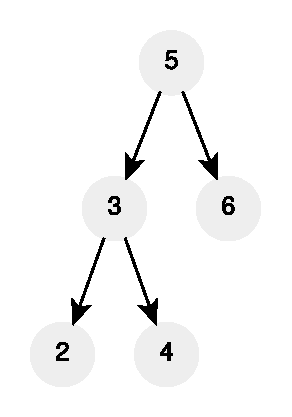
\includegraphics[width=\textwidth]{sources/nqueens/images/example1}
%   \caption[Sample short cpation]{Sample Caption}. \label{fig:nqueens:example1} \end{figure}

\chapter{N-Queens}
\label{ch:nqueens}
\section*{Introduction}
In this chapter we are going to discuss a problem that is more known because of one of its
specialization, namely the eight queen puzzle where you are challenged with the problem of placing
eight chess queens on an $8 \times 8$ chessboard so that no two queens threaten each other
requiring, therefore that no two queens share the same row, column or diagonal.

The n-queens is a classical and old problem which is used as an example of a simple but definitely
non-trivial problem for various programming techniques such as constraint programming, logic
programming , recursion and even genetic algorithms. In the context of a programming interview, you
should aim for precision and for outlining the solution strategy clearly while solving it. The
interview is very likely expecting you to be comfortable with the problem already, and possibly with
the solution but he want to see how well you can explain and materialize into code all the steps
that are in between a purely brute-force and a more sophisticated solution.

\begin{figure}
	 \centering 
	 \newgame
	 \def\myfen{4q3/6q1/3q4/q7/2q5/7q/5q2/1q6 w - - 0 1}
	 \chessboard[labelbottomformat=\arabic{filelabel}, %bottom labels are numbers
	 showmover=false, %do not show the mover
	 setfen=\myfen] \caption{Example of solution of the $8$-queens problem}.
	  \label{fig:nqueens:chessboard}
\end{figure}


\section{Problem statement}
\begin{exercise}
\label{example:nqueens:exercice1}
The $n$-queens puzzle is the problem of placing $n$ queens on an $n \times n$ chessboard in such a
way that no two queens can attack each other. A queen can attach any piece along its row, column or
diagonals. Write a function that given an integer $1 \leq n$, returns all solutions to the
$n$-queens puzzle.

A solution is to be returned as a snapshot of the chessboard. A snapshot of the board is an array of
$n$ strings, each representing a row, where an empty cell is denoted by the symbol '.' and a cell
occupied by a queen by the letter 'Q'.

For instance \textit{"xxxx"} is the snapshot of the board shown in Figure
\ref{fig:nqueens:chessboard}. 

	%example1
	\begin{example}
		\label{example:nqueens:example1}
		\hfill \\
		Given $n=4$ the function returns an array containing the following snapshots:
		\begin{enumerate}
			\item \texttt{[".Q..","...Q","Q...","..Q."]} (see Figure
			\ref{fig:nqueens:chessboard4x4_1})
			\item \texttt{["..Q.","Q...","...Q",".Q.."]} (see Figure
			\ref{fig:nqueens:chessboard4x4_2})
		\end{enumerate}
		
	\end{example}

\end{exercise}

\begin{figure}[t]
	\centering
	\begin{subfigure}[t]{0.48\textwidth}
		\centering
		\def\myfen{1q2/3q/q3/2q1 w - - 0 1} \chessboard[labelbottomformat=\arabic{filelabel},
		%bottom labels are numbers
					maxfield=d4, % set board size
					showmover=false, %do not show the mover
					setfen=\myfen]
		\caption{}
		 \label{fig:nqueens:chessboard4x4_1}
	 \end{subfigure}
	\hfill
	\begin{subfigure}[t]{0.48\textwidth}
		\centering
		\def\myfen{2q1/q3/3q/1q2 w - - 0 1} \chessboard[labelbottomformat=\arabic{filelabel},
		%bottom labels are numbers
					maxfield=d4, % set board size
					showmover=false, %do not show the mover
					setfen=\myfen]
		\caption{}
		 \label{fig:nqueens:chessboard4x4_2}
	 \end{subfigure}

	\caption{Solutions to the $4$-queens problem.}.
	 \label{fig:nqueens:chessboard4x4}
\end{figure}

\section{Discussion}
\label{nqueens:sec:discussion}
The queen (\symqueen) in the game of chess is the most powerful piece as it is able to move any
number of unoccupied cells vertically, horizontally and diagonally, as shown in Figure
\ref{fig:nqueens:queen_movements}. Its movement pattern is the combination of the moves of the rook
(\symrook) and the bishop (\symbishop).

\begin{figure}
	\centering 
	\def\myfen{8/8/8/8/8/3q3/8/8 w - - 0 1} \chessboard[setfen=\myfen, pgfstyle=straightmove,
	arrow=stealth, linewidth=.3ex, padding=2ex, color=black!75!white, shortenstart=1.15ex,
	showmover=false, markmoves={d3-h7,d3-a6,d3-b1,d3-f1,d3-d8,d3-d1,d3-a3,d3-h3}] 
	\caption{Moves of a chess queen.}
	 \label{fig:nqueens:queen_movements}
\end{figure}



\subsection{Brute-force}
\label{nqueens:sec:bruteforce}

A purely brute-force approach can be incredibly expensive as there are ${n^2 \choose n}$ possible
ways of placing $n$ queens on a $n \times n$ board. For an $8 \times 8$ board that translates to a
whopping $4426165368$ possible arrangements but only $92$ distinct solutions! This approach is
extremely easy to implement as the only thing that is necessary is to be able to enumerate all the
queens' arrangements and filtering out the ones in which a queen can attack any of the others. This
last step can be done by checking, for each queen, whether another queen is places in its row,
column or diagonals. Listing \ref{list:nqueens:bruteforce} shows an implement of this idea where we
use the function \inline{nqueen_bruteforce} as a driver and the function
\inline{nqueen_bruteforce_helper} to generate all possible arrangements for the queens and the
function \ref{is_valid_solution} to evaluate it. An arrangement is a combination of size $n$ taken
from a list of all possible board cells \inline{location}. The function
\inline{nqueen_bruteforce_helper} works similarly to the function \inline{all_combinations} in
Listing \ref{list:min_difficulty_job_scheduler:combinations} (at page
\pageref{list:min_difficulty_job_scheduler:combinations} in Chapter
\ref{ch:min_difficulty_job_scheduler}) with the difference that the combination is just evaluated to
see if it is a valid solution and only saved if such test is positive.

Function \ref{is_valid_solution} takes care of validating a solution candidate by checking whether
no two queens placed at locations $(a,b)$ and $(c,d)$ do not share the same:
\begin{itemize}
	\item row (when $a = c$  or $a-c=0$)
	\item column (when $b = d$  or $b-d=0$) 
	\item diagonal (either when:
	\begin{itemize}
		\item $a-c = b-d$, meaning that you can reach $(c,d)$ by advancing by the same number of
		rows and column from $(a,b)$ 
		\item $|a-c| = |b-d|$ and $\sign{(a-c)} \leq \sign{(b-d)}$  which has the geometrical
		intepretation that you can  reach $(c,d)$ by advancing by the same number of rows and column
		from $(a,b)$ but in opposite directions: advance $k$ rows and step back $k$ columns or the
		other way round.
	\end{itemize} 
\end{itemize}

\lstinputlisting[language=c++, caption={Bruteforce solution to the n-queens problem.},label=list:nqueens:bruteforce]{sources/nqueens/nqueens_solution1.cpp}

\subsection{One row one queen}
\label{nqueens:sec:onerowonequeen}
The purely bruteforce solution goes through a number of arrangements that are by construction invalid. 
We know that a queen placed on a given row $k$ makes it impossible for another queen to
be placed in the same row. 
Therefore, we can place a queen at row $i$ and then try to place the remaining queens in the rest of the board without considering row $i$ again. 
This approach significantly reduces the number of possible arrangements as there are $n^n$ ways of doing so ($n$ choices per each row).
Listings \ref{list:nqueens:oneperrow} shows an implementation of this idea.

\lstinputlisting[language=c++, caption={Solution to the n-queens problem where we do not place more than one queen on the same row.},label=list:nqueens:oneperrow]{sources/nqueens/nqueens_solution2.cpp}


\subsection{One queen per column}
\label{nqueens:sec:onequeenpercolumn}
The approach discussed in Section \ref{nqueens:sec:onerowonequeen} is still 
generating arrangements that are invalid by construction and the reason is that
it tries all those arrangements where two queens are placed on the same column. 
We can prevent this from happening by using the  reusing the idea of placing one queen per row
and by also placing one queen per column. This can be achieved by using 
one of the $n!$ permutations of the numbers  $0,1,2,\ldots n-1$ as indices to place a queen on each row.
We can then reject a candidate solution only by looking at the diagonal attacking positions. 
Listing \ref{list:nqueens:oneperrowcolumn} shows an implementation of this idea that uses the 
\inline{std::next_permutation} function to generate the permutations.
This approach is in practice significantly faster than the ones presented above.

\lstinputlisting[language=c++, caption={Solution to the n-queens problem where we do not place more than one queen on the same row and column.},label=list:nqueens:oneperrowcolumn]{sources/nqueens/nqueens_solution3.cpp}



\subsection{Brute-force Revisited}
\label{nqueens:sec:bruteforcerevisited}
The purely bruteforce approach shown in Section \ref{nqueens:sec:bruteforce} can be improved quite dramatically by using an early prunining tecnique that
does not wait to reject a given arrangements until all the queens are places, but does so as soon as a conflict is found, even on a partial candidate solution.
Surprisingly this can be achieved with minimal changes to the Listing \ref{list:nqueens:bruteforce} by adding a call to 
\inline{is_valid_solution(sol_candidate)} every-time an element is added to the candidate solution list.
Listing \ref{list:nqueens:bruteforcerevised} shows how this modified version of the brute-force approach above can be implemented.
Notice that the function \inline{can_add_queen} is pretty much a copy and paste of the function \inline{is_valid_solution} with the (crucial)
difference that it only checks whether is it legal to add a queen at the position specified by its second argument when you have already a number of queens placed in the board which positions are defined in its first parameter.
This solution has performance that are very much comparable to the fastest one shown in this chapter, Listing \ref{list:nqueens:oneperrowcolumn}.

\lstinputlisting[language=c++, caption={Revised brute-force solution to the n-queens problem optimized by using  an early prunining tecnique.},label=list:nqueens:bruteforcerevised]{sources/nqueens/nqueens_solution4.cpp}
